%Template pembuatan proposal skripsi.
\documentclass{jtetiproposalskripsi}

%-----------------------------------------------------------------
%Disini awal masukan untuk data proposal skripsi
%-----------------------------------------------------------------
\titleind{RUNTIME MONITORING UNTUK TESTING BERBASIS MODEL
PADA SISTEM TERDISTRIBUSI}

\fullname{NOVAN AGUNG SUCAHYO}

\idnum{NIM : 1110651206}

\approvaldate{11 Januari 2015}

\degree{Sarjana Teknik Elektro}

\yearsubmit{2015}

\program{Teknik Informatika}

\headprogram{Eko Fajar, S.Kom}

\dept{Teknik Informatika}

\firstsupervisor{Eko Fajar Y, S.Kom}
\firstnip{1976 0501 2002 12 1 002}

\secondsupervisor{Triawan Adi Cahyanto, M.Kom}
\secondnip{1977 0131 2002 12 1 003}


%-----------------------------------------------------------------
%Disini akhir masukan untuk data proposal skripsi
%-----------------------------------------------------------------

\begin{document}

\cover

\approvalpage

%-----------------------------------------------------------------
%Disini akhir masukan untuk muka skripsi
%-----------------------------------------------------------------

%-----------------------------------------------------------------
%Disini awal masukan Intisari
%-----------------------------------------------------------------
\begin{abstractind}
Dampak dan pengaruh dari perkembangan teknologi saat ini semakin meningkat di berbagai perusahaan, organisasi maupun masyarakat. Kemajuan teknologi begitu cepat sehingga dapat memperbaharui sistem kerja yang masih manual menjadi terkomputerisasi. Suatu sistem yang dapat membantu pengerjaan segala bentuk kegiatan perusahaan atau organisasi misalkan melakukan input, pemrosesan data dan output data sehingga didapatkan hasil yang tepat dan akurat. Pada lingkungan perusahaan tersebut sebuah sistem yang didistribusikan memerlukan sebuah pemantauan kinerja atau waktu pemrosesan data dengan proses pendekatan terhadap sebuah sistem.

Proses pendekatan pada perusahaan tersebut dapat dilakukan dengan mengembangkan teknik untuk pemodelan interaksi, yang memberikan cara untuk mengetahui secara resmi apa yang terjadi dalam sebuah sistem. Fitur penting dari pendekatan tersebut adalah pemantauan interaksi. Hal ini menjembatani antara sistem nyata dan model. Kita melihat \emph{monitoring run-time} adalah sebagai alternatif terbaik. 

Dalam makalah ini telah memperkenalkan pendekatan berbasis model untuk pengujian sistem terdistribusi . Pendekatan ini memiliki penekanan kuat pada aplikasi praktis dan didasarkan pada pemantauan run-time sistem. Untuk mengaktifkan pemantauan tersebut dalam sistem perusahaan nyata kita mengembangkan lingkungan pengujian transparan yang bertindak sebagai pengamat untuk interaksi antara komponen sistem terdistribusi . Kita menggunakan aplikasi yang sudah ada yaitu berbasis \emph{open-source platform} teknologi \emph{ESB platform} untuk lingkungan pengujian. Telah dikelompokkan bahwa pendekatan untuk generasi model sistem terdistribusi yang didasarkan pada mengamati pola perilaku dari masing-masing komponen . Model ini composable dari masing-masing komponen . Model yang kompatibel ini dapat digunakan di seluruh tahapan dari proses pengujian. Hasil pengamatan pada masing masing komponen bisa dilihat langsung pada tiap komponen yang terdapat pantauan yang sudah dipasangkan pada tiap komponen tersebut. Komponen bisa lebih ringan dalam memonitoring komponen dibawahnya tanpa harus memonitoring semua komponen dibawahnya sekaligus.

\bigskip
\textbf{Kata kunci} : Sistem, Alternatif, \emph{open-source platform}, \emph{ESB platform}, Model, Kompatibel.
\end{abstractind}
%-----------------------------------------------------------------
%Disini akhir masukan Intisari
%-----------------------------------------------------------------

\tableofcontents
\addcontentsline{toc}{chapter}{DAFTAR ISI}
\selectlanguage{bahasa}\clearpage\pagenumbering{arabic}\setcounter{page}{1}

%-----------------------------------------------------------------
%Disini awal masukan untuk Bab
%-----------------------------------------------------------------
\chapter{LATAR BELAKANG}

\section{Latar Belakang Masalah}
Dampak dan pengaruh dari perkembangan teknologi saat ini semakin meningkat  di berbagai perusahaan, organisasi maupun masyarakat. Kemajuan teknologi begitu cepat sehingga dapat memperbaharui sistem kerja yang masih manual menjadi terkomputerisasi. Suatu sistem yang dapat membantu pengerjaan segala bentuk kegiatan perusahaan atau organisasi misalkan melakukan input, pemrosesan data dan output data sehingga didapatkan hasil yang tepat dan akurat.

Lingkungan perusahaan biasanya sering dibagi antara beberapa domain teknologi , masing-masing terbentuk dengan berbagai jenis  solusi seperti broker integrasi , server aplikasi atau layanan bus . Oleh karena itu lingkungan perusahaan  secara keseluruhan sangat didistribusikan . 
Pada lingkungan perusahaan tersebut sebuah sistem yang didistribusikan memerlukan sebuah pemantauan kinerja atau waktu pemrosesan data dengan proses pendekatan terhadap sebuah sistem.  Proses pendekatan tersebut dapat dilakukan dengan dua cara yaitu cara yang pertama dapat dilakukan dengan mencoba untuk mengembangkan kerangka pengujian yang menawarkan sebuah sistem tersebut dapat mengamati dan kontrol terhadap interaksi dalam lingkungan pengujian. Proses pendekatan yang kedua yaitu mengembangkan teknik untuk pemodelan interaksi, yang memberikan cara untuk mengetahui secara resmi apa yang terjadi dalam sebuah sistem.

Fitur penting dari pendekatan tersebut adalah pemantauan interaksi. Hal ini menjembatani antara sistem nyata dan model. Kita melihat monitoring run-time adalah sebagai alternative terbaik.

\section{Perumusan Masalah}
\begin{enumerate}[a.]
\begin{singlespace}
\itemsep0em
\item Bagaimana cara pendekatan praktis untuk mengelola proses pengujian untuk  sistem terdistribusi ?
\item Dan Bagaimana cara kerja dari transparanted test envirountment ?
\end{singlespace}
\end{enumerate}

\section{Batasan Masalah}
Batasan masalah dalam proyek tugas akhir ini penulis membatasi permasalahan dalam memonitoring prosedur  sistem terdisrtibusi perusahaan.

\section{Tujuan Penelitian}
\begin{enumerate}[a.]
\begin{singlespace}
\itemsep0em
\item Mengetahui cara pendekatan praktis untuk mengelola proses pengujian untuk  sistem terdistribusi.
\item Mengetahui cara kerja dari dari transparanted test envirountment.
\end{singlespace}
\end{enumerate}

\section{Manfaat Penelitian}
\subsection{Bagi Penulis}
Dapat menambah pengetahuan dan wawasan serta dapat mengaplikasikan dan mensosialisasikan teori yang telah diperoleh selama perkuliahan.

\subsection{Bagi penulis selanjutnya}
Dengan penelitian ini diharapkan dapat menjadi wwawasan pengetahuan mengenai metode monitoring sistem terdistribusi bagi penulis selanjutnya yang tertarik untuk meneliti metode monitoring sistem terdistribusi lebih dalam.

\subsection{Bagi Masyarakat}
Diharapkan menghasilkan informasi yang dapat dibahas pertimbangan dalam melakukan kegiatan pada perusahaan.


%-------------------------------------------------------------------------------
\chapter{TINJAUAN PUSTAKA}                

\section{Sistem Terdistribusi}
	 Sistem merupakan kumpulan dari subsistem atau komponen atau elemen yang mempunyai tujuan yang sama yaitu untuk mencapai suatu sasaran atau tujuan yang diinginkan. Subsistem atau komponen atau elemen adalah bagian dari suatu sistem yang saling berkaitan dan saling mempengaruhi antara satu bagian dengan bagian yang lain dalam sistem tersebut. Secara sederhana sistem merupakan suatu jaringan yang saling bekerja sama untuk mencapai suatu tujuan yang telah ditentukan sebelumnya. sebuah sistem terdiri dari input dan output dimana input tersebut memberi masukan kedalam suatu sistem kemudian oleh sistem tersebut input diubah menjadi output yang berguna dan bernilai bagi aktor.
	 
Distribusi artinya proses yang menunjukkan penyaluran barang dari produsen sampai ke tangan masyarakat konsumen. Produsen artinya orang yang melakukan kegiatan produksi. Konsumen artinya orang yang menggunakan atau memakai barang/jasa dan orang yang melakukan kegiatan distribusi disebut distributor. Distribusi merupakan kegiatan ekonomi yang menjembatani kegiatan produksi dan konsumsi. Berkat distribusi barang dan jasa dapat sampai ke tangan konsumen. Dengan demikian kegunaan dari barang dan jasa akan lebih meningkat setelah dapat dikonsumsi. Dari apa yang baru saja diuraikan, tampaklah bahwa distribusi turut serta meningkatkan kegunaan menurut tempatnya (place utility) dan menurut waktunya (time utility).

\begin{figure}[ht!]
  \centering
    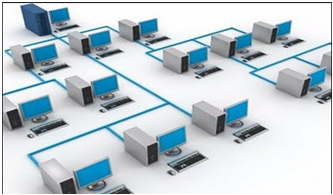
\includegraphics{gambar/1}
    \caption{Sistem Terdistribusi.}
    \label{wsn}
\end{figure}

Sistem Terdistribusi adalah sebuah sistem dimana komponen hardware atau software-nya terletak dalam suatu jaringan komputer dan saling berkomunikasi dan berkoordinasi mengunakan message pasing. sebuah sistem yang terdiri dari kumpulan dua atau lebih komputer dan memiliki koordinasi proses melalui pertukaran pesan synchronous atau asynchronous. kumpulan komputer independent yang tampak oleh user sebagai satu sistem computer kumpulan komputer autonom yang dihubungkan oleh jaringan dengan software yang dirancang untuk menghasilkan fasilitas komputasi terintegrasi dapat terlihat dari bebarapa pengertian diatas dapat di tarik kesimpulan bahwa sistem terdistribusi adalah sebuah sistem yang terdiri dari beberapa komponen software atau hardware yang independent yang berkomunikasi dan berkoordinasi melalui message parsing baek sinkron maupun asinkron yang telihat satu kesatuan dan dirancang untuk menghasilkan fasilitas komputasi terintegrasi.


\section{Transparent envirountment}

Dasar dari pendekatan ini adalah lingkungan yang dapat diamati . Sementara mengevaluasi sifat dari komponen yang diuji dan menganggap bahwa interaksi antara komponen tersebut diamati.

\begin{figure}[ht!]
  \centering
    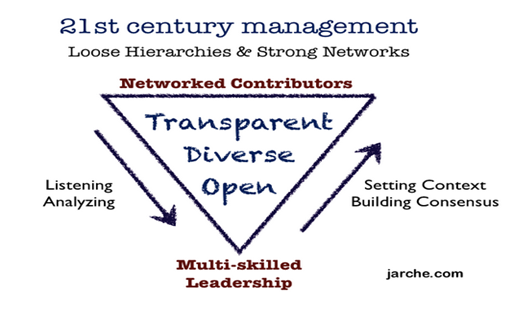
\includegraphics{gambar/2}
    \caption{Transparent envirountment.}
    \label{wsn}
\end{figure}

Kontributor Jaringan (full-time, paruh waktu, kontraktor) perlu bekerja sama dalam lingkungan jaringan yang memfasilitasi kerjasama dan kolaborasi. Inilah sebabnya mengapa narasi kerja dan PKM akan menjadi keterampilan yang penting, sebagai tim kerja surut dan aliran sesuai dengan kebutuhan, tetapi jaringan harus tetap terhubung dan tangguh. Fungsi utama dari para pemimpin (berpikir kepemimpinan pelayan) akan mendengarkan dan menganalisis apa yang terjadi. Dari pemandangan luas, mereka dalam peran kepemimpinan dapat membantu mengatur konteks kerja sesuai dengan perubahan lingkungan dan kemudian bekerja pada membangun konsensus. Kekuatan jaringan sosial, seperti listrik, pasti akan berubah hampir setiap model bisnis. Pemimpin perlu memahami pentingnya arsitektur organisasi. Bekerja cerdas di tempat kerja masa depan dimulai dengan mengorganisir untuk merangkul jaringan, mengelola kompleksitas, dan membangun kepercayaan.

\section{HTTP Sniffing}
\begin{figure}[ht!]
  \centering
    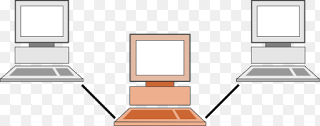
\includegraphics{gambar/3}
    \caption{HTTP Sniffing.}
    \label{wsn}
\end{figure}
Sniffing merupakan teknik pemantauan sebuah jaringan computer yang dapat digunakan pada jaringan komputer. Terdapat dua tipe sniffing yaitu passive sniffing dan active sniffing.

HTTP Sniffing merupakan pemantauan pada pengiriman data yang menggunakan koneksi HTTP. Data yang dikirimkan lalu lalang di jaringan dalam bentuk plain text.
Passive sniffing ini memerlukan program sniffer yang akan merubah kartu jaringan agar dapat melihat dan mencatat semua data yang dilaluinya.

Active sniffing sulit dilakukan. Karena sniffing ini komputer harus saling terhubung.  Sehingga data yang dikirimkan terhubung ke komputer pusat. Dengan demikian pihak dari programmer aktif memantau lalu lintas data pada jaringan komputer.
 
Langsung ke inti, Spotflux adalah sebuah aplikasi yang berperan sebagai server proxy yang menjembatani client ( dalam hal ini anda sebagai user ) dengan internet. Bisa diibaratkan Spotflux adalah pihak ketiga yang berdiri ditengah-tengah antara kedua pihak yang saling berhubungan dan berfungsi sebagai perantara, sedemikian rupa sehingga pihak pertama dan pihak kedua tidak secara langsung berhubungan. Spotflux juga membantu mengembangkan keamanan dengan memfilter beberapa konten web dan software merusak.

\section{ESB Platforms}
\begin{figure}[ht!]
  \centering
    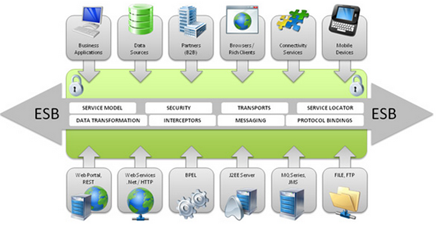
\includegraphics{gambar/4}
    \caption{ESB Platforms.}
    \label{wsn}
\end{figure}
ESB (Enterprice Service Bus ) merupakan infrastruktur untuk koneksi layanan SOA dan pertukarran pesan. Ungsionalitas utama ESB adalah melakukan rute, transformasi protocol serta transformasi pesan atau data. Dengan adanya fungsi transformasi protocol dan pesan pada ESB ini maka ketidak sesuaian protocol dan data dapat diatasi. ESB juga memudahkan koneksi dan mediasi, menyederhanakan integrasi serta memudahkan pemnggunaan ulang komponen komponen layanan, sehingga skalabilitas integrasi menjadi tinggi.

	ESB diperlukan untuk koneksi ke beberapa sumber daya TI. ESB harus fleksibel untuk menggabungkan dan memasang ulang komponen sesuai dengan perubahan kebutuhan bisnis. ESB melakukan koneksi komponen yang terikat longgar, sehingga menyediakan kemampuan untuk mengintegrasikan sistem ke dalam SOA dan mendeploy secara bertahap.
	
	ESB menyediakan infrastruktur komunikasi antar layanan yang kuat, dapat diandalkan, aman dan dapat diperluas. ESB juga menyediakan kendali komunikasi dan kendali atas penggunaan layanan layanan yang mencakup : 

\begin{flushleft}
\item [1]Kemampuan  menangkap pesan yang memungkinkan untuk menangkap pesan request untuk layanan  layanan dan pesan response dari layanan. Serta memberikan pemrosesan tambahan. Dengan cara ini ESB dapat bertindak sebagai intermediary.
\item [2]Kemampuan routing, yang memungkinkan ESB melakukan routing pesan ke layanan layanan yang berbeda didasarkan pada isi (content), asal, atau atribut lain.
\item [3]Kemampuan transformasi, yang memungkinkan transformasi pesan sebelum dikirimkan ke layanan layanan. Untuk pesan format XML, trnasformsi semacam ini dilakukan menggunakan XSLT (Extensible Stylesheet Language for Transformations) atau mesin XQuear.
\item[4]Kendali atas deployment, penggunaan dan pemeliharaan layanan layanan. Hal ini memungkinkan adanya logging, profiling, load balancing, performance tunning, ongkos penggunaan layanan layanan, distributed deployment, on the fry reconfiguration , dsb.
\end{flushleft}

Solusi untuk masalah integrasi dapat ditemukan dalam Arsitektur Software. Arsitektur yang ideal harus sedemikian rupa sehingga sistem yang terlibat harus menangkap dan bereaksi terhadap peristiwa (EDA: Event Driven Architecture) dan akan juga berorientasi pada layanan (SOA: Service Oriented Architecture).

\section{Service Mix}
CHORUS merupakan keluarga dari sistem operasi berbasis mikro-kernel untuk mengatasi kebutuhan komputasi terdistribusi tingkat tinggi di dalam bidang telekomunikasi, internetworking, sistem tambahan, realtime, sistem UNIX, supercomputing, dan kegunaan yang tinggi. Multiserver CHORUS/MiX merupakan implementasi dari UNIX yang memberi kebebasan untuk secara dinamis mengintegrasikan bagian-bagian dari fungsi standar di UNIX dan juga service dan aplikasi-aplikasi di dalamnya.

Apache ServiceMix merupakan open source didistribusikan ESB dibangun dari bawah ke atas di Java Integrasi Bisnis (JBI) spesifikasi JSR 208 dan dirilis di bawah lisensi Apache. Tujuan dari JBI adalah untuk memungkinkan komponen dan jasa untuk diintegrasikan dalam vendor cara yang independen, yang memungkinkan pengguna dan vendor untuk plug and play.
\begin{figure}[ht!]
  \centering
    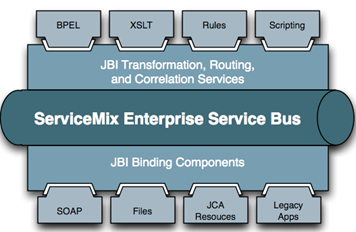
\includegraphics{gambar/5}
    \caption{Service Mix.}
    \label{wsn}
\end{figure}

ServiceMix ringan dan mudah dapat disematkan, telah terintegrasi dengan dukungan Semi dan dapat dijalankan di tepi jaringan (di dalam client atau server), sebagai penyedia ESB mandiri atau sebagai layanan dalam ESB lain. Kita dapat menggunakan ServiceMix di Java SE atau server aplikasi Java EE. ServiceMix menggunakan ActiveMQ untuk memberikan Remoting, clustering, keandalan dan failover didistribusikan. ServiceMix benar-benar terintegrasi ke dalam Apache Geronimo, yang memungkinkan Anda untuk menggunakan komponen dan layanan JBI langsung ke Geronimo. ServiceMix sedang JBI disertifikasi sebagai bagian dari proyek Geronimo. Server aplikasi J2EE lainnya ServiceMix telah terintegrasi dengan termasuk JBoss, Jonas dengan lebih untuk mengikuti.

\section{Synapse}
Synaptic package manager adalah aplikasi untuk mendownload dan menginstal aplikasi dari repository pada linux atau open source.
\begin{figure}[ht!]
  \centering
    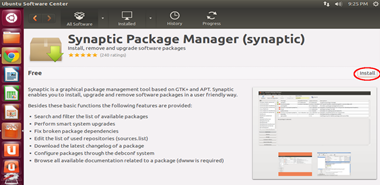
\includegraphics{gambar/6}
    \caption{Synapse.}
    \label{wsn}
\end{figure}

\begin{figure}[ht!]
  \centering
    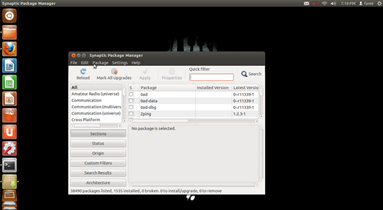
\includegraphics{gambar/7}
    \caption{Synaptic package manager.}
    \label{wsn}
\end{figure}

Synaptic package manager adalah aplikasi untuk mendownload dan menginstall aplikasi dari repository (klo di windows mirip program control panel) jadi jika sudah install aplikasi ini kita semua bisa search dan install aplikasi  lain dengan mudah tanpa harus buka browser untuk mencari aplikasi yang kita perlukan. sebenarnya sudah ada aplikasi yang namanya UBUNTU SOFTWARE CENTER (bagi pengguna ubuntu). tapi sebagian orang menganggap synaptic lebih efektif karena didalamnya kita memilki opsi opsi yang sangat berguna.
Dan kita juga bisa memilih paket yang akan diinstall oleh aplikasi yg akan kita install. jadi kita bisa pilih paket apa saja yang mau kita install dari aplikasi itu, klo tidak perlu tinggal di ilangin centangnya. praktis dan mudah dalam penggunaannya. Sebenarnya mungkin sebagian orang telah tahu tentang hal ini tapi ini ditujukan untuk pengguna linux yang belum berpengalaman tentang linux / Open Source.



%-------------------------------------------------------------------------------
\chapter{METODOLOGI PENELITIAN}

\section{Desain Model}
\begin{figure}[ht!]
  \centering
    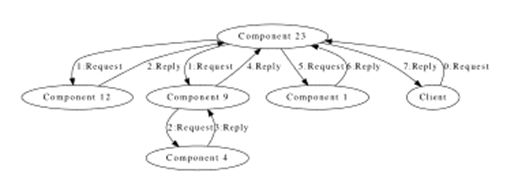
\includegraphics{gambar/8}
    \caption{Desain Model menggunakan interaction Graphr.}
    \label{Desain Model menggunakan interaction Graph}
\end{figure}
Pengamatan yang dilakukan pada interaction graph adalah menyediakan sebuah entitas baru dari sebuah sistem pengamat. Observer harus bisa login , menganalisis , mengubah dan pesan re-route. Dalam jangka waktu tertentu antrian pesan akan diproses yang pada dasarnya berarti bahwa pesan akan dikirim ke tempat tujuan. Pesan yang disampaikan akan di sampaikan secara berurutan dimana jika terdapat pesan A yang dikirim maka pesan selanjutnya atau bisa disebut juga pesan B akan diproses setelah pesan A.

\section{Interaksi Model}
Metode pendekatan awal yang dilakukan adalah dengan menggunakan penciptaan grafik koneksi dari sistem. Seperti yang ditunjukkan pada gambar dibawah.
\begin{figure}[ht!]
  \centering
    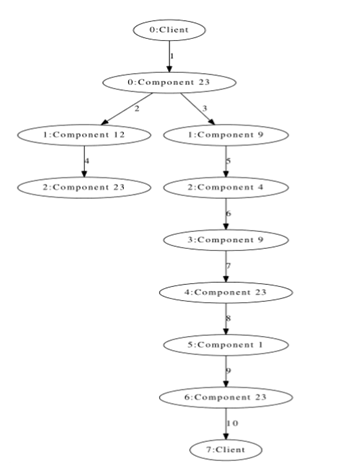
\includegraphics{gambar/9}
    \caption{Interaction Tree.}
    \label{Interaction Tree}
\end{figure}

Yang pada dasarnya adalah hubungan antar komponen. Grafik tersebut dibuat untuk penamtauan pesan dan aliran pada pengamatan dan hampir tidak memerlukan pengolahan selain header pesan di mana tujuan pesan berbeda. Pada gambar tersebut ditunjukkan bahwa pemantauan di letakkan pada setiap bagian komponen sehingga komponen pusat tidak perlu sampai memantau semua komponen dibawahnya. Dengan meletakkan pemantauan pada tiap komponen dapat memantau komponen yang ada pada komponen dibawahnya.

Untuk membuat pohon interaksi kita harus melaksanakan aturan-aturan dasar untuk korelasi pesan :

\begin{enumerate}[a.]
\begin{singlespace}
\itemsep0em
\item Pesan yang bersamaan jika mereka dikirim pada giliran yang sama.
\item Pesan yang berurutan jika pesan kedua dikirim pada gilirannya persis berikutnya dan tujuan dari pesan pertama cocok dengan sumber pesan kedua.
\item Jika tidak ada pesan dalam antrian pengamat , interaksi telah berakhir.
\end{singlespace}
\end{enumerate}

Langkah ketiga adalah untuk menemukan hubungan antara data permintaan aktual dan perilaku komponen. Langkah ini diperlukan untuk model yang bermakna sebagai komponen yaitu data - driven dan langkah tersebut  mungkin tidak hanya tergantung pada jenis data yang masuk , tetapi juga pada semantik . Dengan mengembangkan teknik ini diharapkan untuk dapat menjadi satu set heuristik perilaku untuk menemukan dependensi umum dalam input data , seperti pemesanan pesan dan kesetaraan kelas.

\section{Uji Coba Model}
Langkah terakhir dari pendekatan ini adalah generasi tes berbasis pada model interaksi diperkaya dengan kelas menemukan input. Untuk menguji komposisi tertentu kita perlu untuk memperoleh seperangkat kesatuan dari model yang mampu mencakup semua cabang yang dicapai dari interaksi pohon. 

Tugas ini dapat dicapai jika kita akan mampu menemukan dan berkorelasi masukan yang tepat, masalah di sini adalah bahwa tes ini akan menjadi abstrak yaitu mereka akan berisi deskripsi kelas data, bukan data riil. Data real yang dikumpulkan oleh pengamat dapat menjadi tidak dapat digunakan dalam kasus operasi update, karena data diperbarui tidak lagi mewakili kelas aslinya.
 
Saat ini kita melihat ada pendekatan umum yang mungkin untuk penemuan kasus data konkret, jadi kami menganggap itu dilakukan secara manual. Seperti itu mungkin bahwa beberapa kelas data tidak akan memiliki contoh konkret (karena kami tidak dapat menemukan mereka, bukan karena mereka tidak ada), sangat penting untuk mengembangkan metrik cakupan untuk set tes ini.

\section{Analisa Uji Coba}
Dalam makalah ini telah memperkenalkan pendekatan berbasis model untuk pengujian sistem terdistribusi . Pendekatan ini memiliki penekanan kuat pada aplikasi praktis dan didasarkan pada pemantauan run-time sistem. Untuk mengaktifkan pemantauan tersebut dalam sistem perusahaan nyata kita mengembangkan lingkungan pengujian transparan yang bertindak sebagai pengamat untuk interaksi antara komponen sistem terdistribusi . Kita menggunakan aplikasi yang sudah ada yaitu berbasis open-source platform teknologi ESB platform untuk lingkungan pengujian .

Telah dikelompokkan bahwa pendekatan untuk generasi model sistem terdistribusi yang didasarkan pada mengamati pola perilaku dari masing-masing komponen . Model ini composable dari masing-masing komponen . Model yang composable ini dapat digunakan di seluruh tahapan dari proses pengujian , dari  Formal Workflow Model Berdasarkan dengan  Applied Sciences, unit-testing untuk end-to -end penerimaan pengujian . Fitur utama dari model ini adalah bahwa hal itu memungkinkan mengikat perilaku komponen untuk semantik data input. Hasil pengamatan pada masing masing komponen bias dilihat langsung pada tiap komponen yang terdapat pantauan yang sudah dipasangkan pada tiap komponen tersebut. Komponen bias lebih ringan dalam memonitoring komponen dibawahnya tanpa harus memonitoring semua komponen dibawahnya sekaligus.


\section{Jadwal Kegiatan}
Pada bagian ini diperlihatkan jadwal kegiatan selama penelitian ini berlangsung.  Jadwal disajikan per minggu selama 2 bulan dalam gambar 3.5 dibawah 

\begin{center}
Tabel 3.1. Jadwal Penelitian.
\end{center}
\vspace{-0.5cm}
\begin{figure}[ht!]
  \centering
    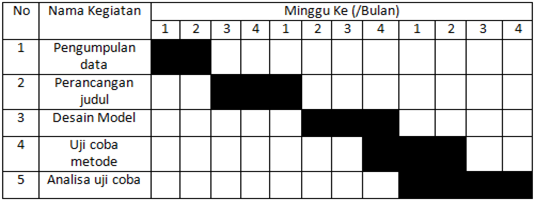
\includegraphics[width=13cm]{gambar/10}
\end{figure}

%-----------------------------------------------------------------
%Disini akhir masukan Bab
%-----------------------------------------------------------------

%-----------------------------------------------------------------
%Disini awal masukan untuk Daftar Pustaka
%-----------------------------------------------------------------
%%\nocite{Abel2010,Guerbas201350}
%%\bibliography{research-plan}
%%\bibliographystyle{plainnat}
\begin{thebibliography}{9}

\bibitem[satu(2013)]{satu01}
1.  A. Ferrara. L. Sapienza, and V. Salaria. “Web Services : a Process Algabra Approach.” pp. 242-251.

\bibitem[dua(2013)]{dua02}
2.	A. Textor. M. Schmid. J. Schaefer. And R. Kroegar. “SOA Monitoring Based on a Formal Workflow Model with Constrations.” Applied Sciences. pp.47-53.2009.

\bibitem[tiga(2013)]{tiga03}
3.	C. Hewitt, “Actor Model Of Computation : Scalable Robust Information Systems.” Pp. 1-29, 2011.

\bibitem[empat(2013)]{empat04}
4.	I. Burdonov and A. Kosachev , “Conformance testing based on a state relation.” Proceedings of the institute for System Programming  of RAS. vol.  18. pp. 183-220, 2010.

\bibitem[lima(2013)]{lima05}
5.	J. Tretmans, “Model based Testing with Labelled Transition Systems.”

\bibitem[enam(2013)]{enam06}
6.	M. Odersky and L. Spoon. “Programming in Scala.” 2008.

\bibitem[tujuh(2013)]{tujuh07}
7.	M. Sirjani and M.M. Jaghoori, “Ten Years of Analizing Actor : Rebeca Experience.” 

\end{thebibliography}
\addcontentsline{toc}{chapter}{DAFTAR PUSTAKA}
%-----------------------------------------------------------------
%Disini akhir masukan Daftar Pustaka
%-----------------------------------------------------------------

\end{document}